\textbf{Metadata Intensive Workloads -- }
We use the synthetic {\it mdtest} benchmark to generate a three-phase workload:
The first phase creates 5 million
zero-files in a single shared directory \cite{ceph:weil06, GIGA11}.
The second phase performs $stat()$ on random files in this large directory.
The third phase deletes all files in this directory in a random order.
%Each phase uses all the 160 clients to issue operations concurrently in a
%random order.

We compare the performance of native PanFS and \psys for this benchmark.
However, to ensure a fair comparison we cannot compare them directly. This is
because of two reasons: first, a single directory can only utilize one PanFS 
metadata server, and second, PanFS directories can contain at most 1 million 
files.
For a fair comparison, we compare \psys with native PanFS that creates 1 million 
files in 5 different directories owned by 5 different metadata servers.

\begin{figure}[t]  %%%%%%%%%%%%%%%%%%%%%%%
\centerline{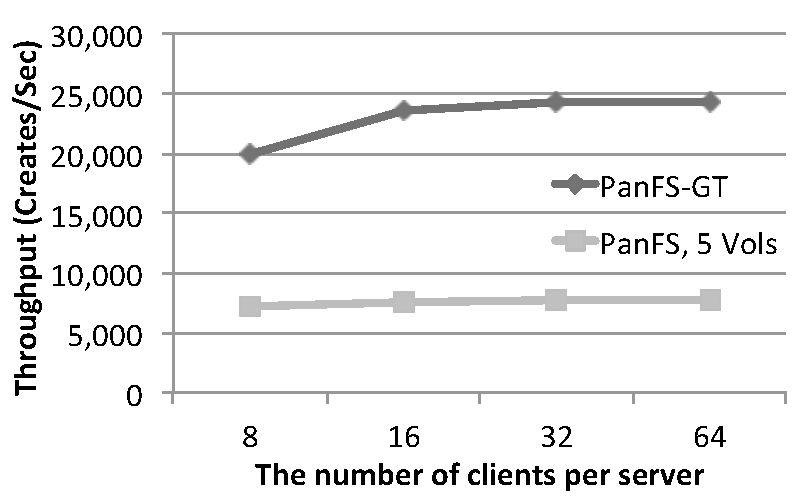
\includegraphics[scale=0.6]{./figs/zero_file_creation_on_panfs}}
\vspace{10pt}
\caption{
\textit{Average throughput during creating five million zero-length files
in one empty directory with different number of clients per test node.
Running 32 and more clients per test node is able to saturate \psys
and original PanFS}
}
%\vspace{10pt}
\hrule
\label{graph:creation_clients}
\end{figure}       %%%%%%%%%%%%%%%%%%%%%%%

\begin{figure}[t]  %%%%%%%%%%%%%%%%%%%%%%%
\centerline{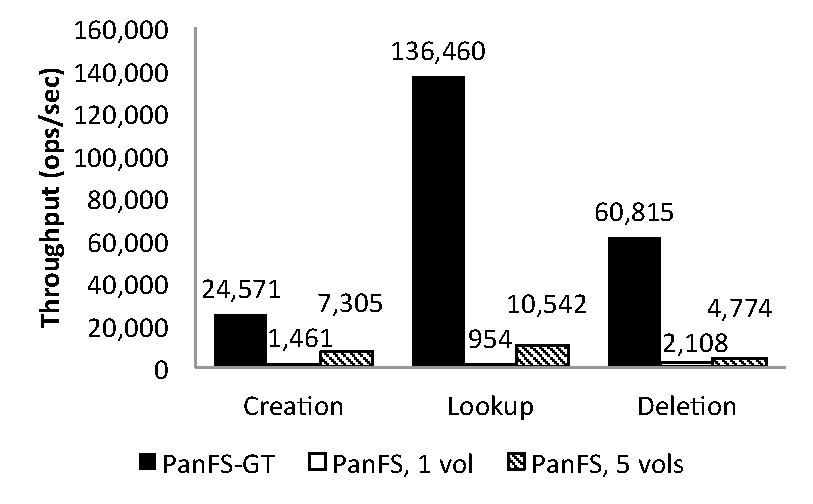
\includegraphics[scale=0.6]{./figs/mdtest}}
\vspace{10pt}
\caption{
\textit{
The average aggregated throughput of different operations in {\it mdtest}
when generating 5 million zero-length files in a single shared directory.
Since PanFS has a hard limit to allow only create 1 million entries
in one directory, the bar showing PanFS with 1 volume only gives
the average throughput for the case of creating 1 million entries.
}
}
%\vspace{10pt}
\hrule
\label{graph:mdtest_ops}
\end{figure}       %%%%%%%%%%%%%%%%%%%%%%%

Figure \ref{graph:creation_clients} shows the aggregated throughput during
the first phase. We vary the number of clients running in each test node
to determine the number of clients needed to saturate both \psys and native
PanFS systems.
Both systems achieve the highest aggregated throughput using 32 or more number 
of clients per node. In all the experiments shown later, by default, we report 
results with 32 clients per test node.
For all cases, \psys is approximately 3.5 times faster than the native PanFS
using 5 volumes. The aggregated peak throughput for the 5-server and
160-client system is about 25,000 file creates per second. 

Figure \ref{graph:mdtest_ops} shows the aggregated throughput of
different operations during the three-phase {\it mdtest} workload.
In addition to the \psys and 5-shelf PanFS, this figure also reports the 
aggregated throughput of creating 1 million files in single-shelf PanFS.
For $lookup$ and $deletion$ workloads, \psys outperforms native PanFS by a
factor to 10 to 15 higher operations per second.
Fast lookup performance results from memory indexing and Bloom filters in \ldb.
For deletion of a key, \ldb essentially just inserts a new entry with the 
deletion mark next to the key to be deleted, and delays the actual deletion in 
later compaction processes.


\begin{figure}[t]  %%%%%%%%%%%%%%%%%%%%%%%
\centerline{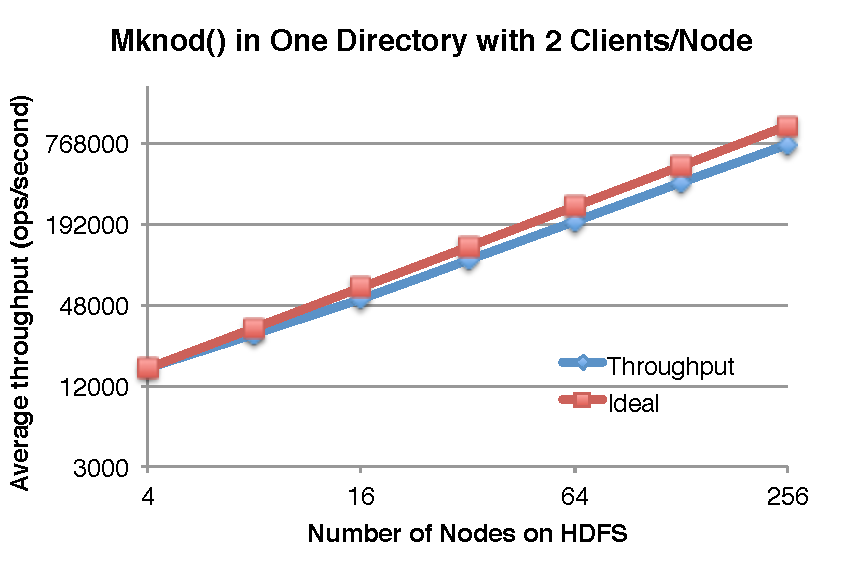
\includegraphics[scale=0.6]{./figs/hdfs_empty_file}}
\vspace{10pt}
\caption{
\textit{Average aggregated throughput during creating 1 million empty files
with different size in one shared directory}
}
%\vspace{10pt}
\hrule
\label{graph:smallfiles}
\end{figure}       %%%%%%%%%%%%%%%%%%%%%%%


\textbf{Small File Workloads -- }

\begin{figure}[t]  %%%%%%%%%%%%%%%%%%%%%%%
\centerline{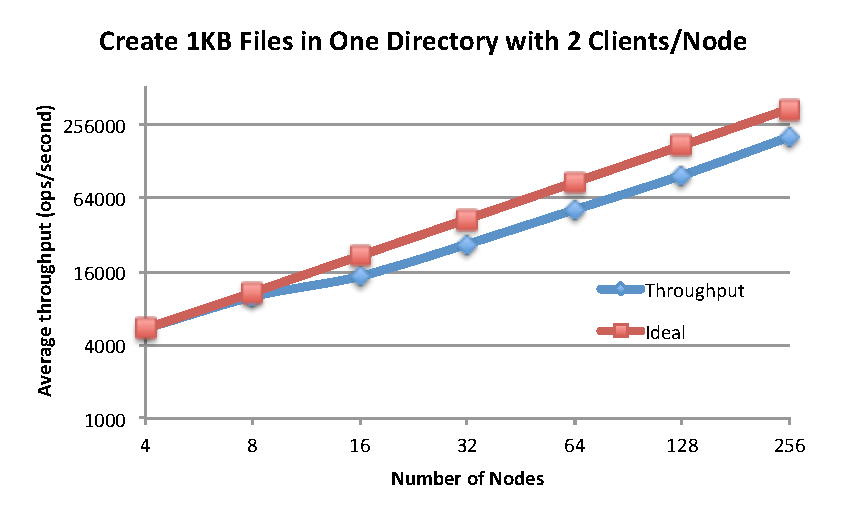
\includegraphics[scale=0.6]{./figs/hdfs_small_file}}
\vspace{10pt}
\caption{
\textit{Average aggregated throughput during creating 1 million small files
per-node with different size in one shared directory}
}
%\vspace{10pt}
\hrule
\label{graph:smallfiles}
\end{figure}       %%%%%%%%%%%%%%%%%%%%%%%


\textbf{Data Intensive Workloads -- }

